\documentclass[12pt,twoside]{article}
\usepackage{geometry}
\geometry{a4paper,landscape,margin=1.2cm}

% svgnames for DimGray color
\usepackage[svgnames]{xcolor}

% images
\usepackage{tikz}
\usetikzlibrary{positioning}
\usetikzlibrary{arrows.meta, decorations.text}


% font stuff
\usepackage{fontspec}
\defaultfontfeatures{Mapping=tex-text,Scale=MatchLowercase}
% use whatever font you want, I just like Noto Sans
\setmainfont{Noto Sans}

% columns
\usepackage{multicol}
% lengths
\setlength{\unitlength}{1mm} % Set the length that numerical units are measured in
\setlength{\parindent}{0pt} % Stop paragraph indentation
% distance between lines
\setlength{\baselineskip}{12pt}%12pt
\setlength{\lineskip}{3.5pt}%3.5pt
\setlength{\lineskiplimit}{2pt}

% dot filling
\renewcommand{\dots}{\ \dotfill{}\ } % Fills in the right amount of dots

% my emph command for glossary
\newcommand{\myem}[1]{\textbf{\ttfamily#1}}

% calculate linewidth in column
\newlength{\mylinewidth}
\setlength{\mylinewidth}{\dimexpr\linewidth-\columnsep-3pt\relax}

% command for colored command box
\newcommand{\cmdbox}[1]{\par\noindent\colorbox{Gainsboro}
{\parbox{\the\mylinewidth}{\small\ttfamily#1}}}

% command for a shortcut/command and its explanation
\newcommand{\command}[2]{
\parbox{\the\mylinewidth}{% put both in a parbox so we don't get column/page breaks between a command and its explanation
\cmdbox{#1}\vspace{1.5pt}
#2}
}

 % section title and maketitle
\newcommand{\sectiontitle}[1]{\vspace*{8pt}\textsc{\textbf{#1}} \ \textcolor{DarkGray}{\hrulefill}\\} % Custom command for subsection titles
\newcommand{\subsectiontitle}[1]{\textcolor{Black}{\textbf{#1}}\\} % Custom command for subsection titles

\makeatletter
\renewcommand{\maketitle}{{\centering{\Large\bfseries\@title}}}
\makeatother

\pagestyle{empty}

\title{Git Cheat Sheet}
\begin{document}
\begin{multicols*}{2}
\maketitle

\sectiontitle{Setup}
\command{git config --global user.name "<firstname lastname>"\\ git config --global user.email "<valid-email>"}{set name and email to be associated with version history}
\command{git config --global colors.ui auto}{set automatic command line coloring}
\command{git config --global alias.<alias-name> "<git-command>"}{define a shortcut/alias for a git command}
\command{git config --system core.editor <editor>}{set default text editor used by commands}
\command{git config --global --edit}{open global configuration file in text editor}
\command{git init}{initialize an existing directory as git repository}
\command{git clone <url>}{retrieve a repository from a hosted location via URL}
\command{git clone --branch <branch-name> <url>}{clone a specific branch from the remote repository}

\sectiontitle{Gitignore}
\command{logs/\\*.notes\\pattern*/}{save a file with desired patterns as {\ttfamily .gitignore} with either direct string matches or wildcard globs}
\command{git config --global core.excludesfile <file>}{system wide ignore pattern for all local repositories}

\sectiontitle{Rewrite history}
\command{git rebase <branch>}{apply any commits of current branch ahead of specified one}
\command{git reset --hard <commit>}{clear staging area, rewrite working tree from specified commit}

\vfill\null
\columnbreak
\sectiontitle{Stage \& snapshot}
\command{git status}{show modified files in cwd, staged for next commit}
\command{git add <file>}{add a file as it looks now to your next commit (stage file)}
\command{git reset <file>}{unstage a file while retaining the changes in cwd}
\command{git diff}{show diff between cwd and staging area}
\command{git diff --staged}{show diff between staged changes and last commit}
\command{git commit -m "<message>"}{commit your staged content as a new commit snapshot}
\command{git commit --amend}{replace the last commit with the staged changes and last commit combined. use with nothing staged to edit the last commit's message}
\command{git clean -f}{remove unversioned files}

\sectiontitle{Working with branches}
\command{git branch}{list your branches. a * marks the currently active branch}
\command{git branch <branch-name>}{create a new branch at the current commit}
\command{git checkout}{switch to another existing branch and check it out into cwd}
\command{git checkout -b <branch-name>}{create and check out a new branch with branch-name}
\command{git merge <branch-name>}{merge the specified branch's history into the current one}
\command{git branch-d <branch-name>}{delete the specified branch}

\vfill\null
\columnbreak
\sectiontitle{Temporary commits / stashes}
Temporarily store modified, tracked files in order to change branches\\
\command{git stash}{saved modified and staged changes}
\command{git stash list}{list stack-order of stashed file changes}
\command{git stash pop}{apply and remove most recent stash from stash stack}
\command{git stash drop}{discard most recent stash of stash stack}

\sectiontitle{Path changes}
\command{git rm <file>}{delete the file from project and stage the removal for commit}
\command{git mv <existing path> <new path>}{change an existing file path and stage the move}
\command{git log --stat -M}{show all commit logs with indication of any paths that moved}

\sectiontitle{Inspect \& compare}
\command{git log}{show commit history for currently active branch}
\command{git log branchB..branchA}{show the commits on branchA that are not on branchB}
\command{git log --follow <file>}{list version history for a file, including renames}
\command{git diff <first-branch>..<second-branch>}{show the diff between two branches}
\command{git show <commit>}{show metadata and content changes of the specified commit}
\command{git blame <file>}{show who edited each line of a file}

\vfill\null
\columnbreak
\sectiontitle{Remote repositories}
\command{git remote add <alias> <url>}{add a git URL as an alias}
\command{git fetch <alias>}{fetch down all the branches from that git remote}
\command{git merge <alias>/<branch>}{merge a remote branch into your current branch to bring it up to date}
\command{git push <alias> <branch>}{transmit local branch commits to the remote repository branch}
\command{git pull}{fetch and merge any commits from the tracking remote branch}

\sectiontitle{Glossary}
\myem{HEAD:} representing your cwd, the HEAD pointer can be moved to different branches, tags, or commits when using {\ttfamily git checkout}\\
\myem{index:} different name for the staging area\\

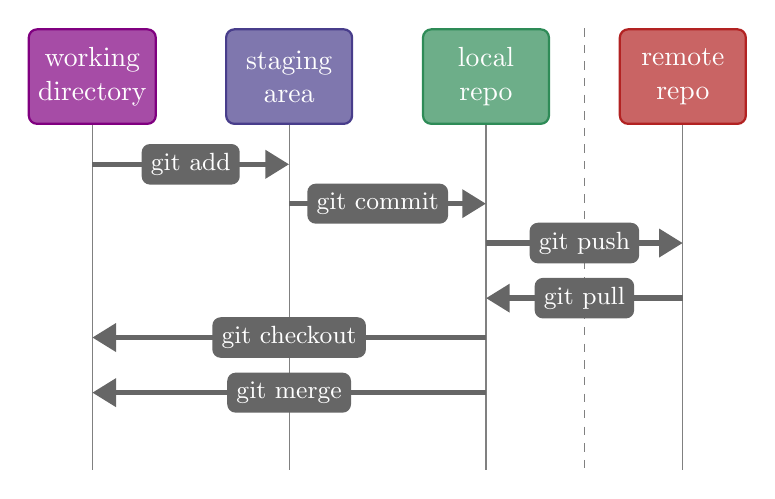
\begin{tikzpicture}[git stage/.style={draw=#1, thick,fill=#1!70, text=white, align=center,
	rounded corners=3pt, minimum height=12mm, minimum width=16mm},
	git stage/.default=black,
	bgline/.style={draw=gray},
	arr/.style={-Triangle[], line width=2pt, draw=black!60},
	tinytext/.style={midway, font=\small, fill=black!60, text=white, line width=0.5pt, rounded corners=3pt}]
	
	\node [git stage=violet] (cwd) at (0,0) {working\\directory};
	\node [git stage=DarkSlateBlue] (staged) at (2.5,0) {staging\\area};
	\node [git stage=SeaGreen] (local) at (5,0) {local\\repo};
	\node [git stage=FireBrick] (remote) at (7.5,0) {remote\\repo};
	
	\draw [bgline] (cwd) -- +(0,-5);
	\draw [bgline] (staged) -- +(0,-5);
	\draw [bgline] (local) -- +(0,-5);
	\draw [bgline] (remote) -- +(0,-5);
	\draw [draw=black!50, dashed] (local.north) +(1.25,0) -- +(1.25, -5.6);
	
	\draw [arr] (cwd.south) +(0,-0.5) -- +(2.5,-0.5) node[tinytext] () {git add};
	\draw [arr] (staged.south) +(0,-1) -- +(2.5,-1) node[tinytext, pos=.45] () {git commit};
	\draw [arr] (local.south) +(0,-1.5) -- +(2.5,-1.5) node[tinytext] () {git push};
	\draw [arr, {Triangle[]}-] (local.south) +(0,-2.2) -- +(2.5,-2.2) node[tinytext] () {git pull};
	\draw [arr, {Triangle[]}-] (cwd.south) +(0,-2.7) -- +(5,-2.7) node[tinytext] () {git checkout};
	\draw [arr, {Triangle[]}-] (cwd.south) +(0,-3.4) -- +(5,-3.4) node[tinytext] () {git merge};
\end{tikzpicture}

\end{multicols*}
\end{document}